
\item Which of the field patterns given below is valid for electric field as well as for magnetic field?
    \begin{center}
        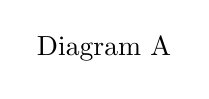
\begin{tikzpicture}
            \node at (0, 0) {Diagram A};
        \end{tikzpicture}
        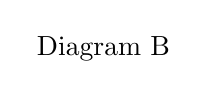
\begin{tikzpicture}
            \node at (0, 0) {Diagram B};
        \end{tikzpicture}
        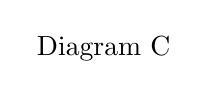
\begin{tikzpicture}
            \node at (0, 0) {Diagram C};
        \end{tikzpicture}
        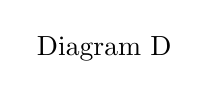
\begin{tikzpicture}
            \node at (0, 0) {Diagram D};
        \end{tikzpicture}
    \end{center}
    \begin{tasks}(2)
        \task (A)
        \task (B)
        \task (C)\ans
        \task (D)
    \end{tasks}
